\section{Results and Discussion}

We applied the equivalent layer methodology to interpolate the residual anomaly (Figure~\ref{gravity}c) onto a regular grid of the geometric topography, as shown in Figure~\ref{final}a. This fit generated a cross-validation R-squared score of 0.952 \citep{Uieda2020}. According to \citet{Vigneresse1990}, a residual-regional separation is considered appropriate when the resulting residual map aligns its zero values contour with the external boundaries of the intrusive body under investigation. Since the residual Bouguer disturbance displayed values close to zero outside the boundaries of the plutonic body it demonstrates the effectiveness of the separation. The negative values occur at the
borders of the SAIC where the granitic rocks outcrop, especially in the southwest
lobe, with a density contrast with the country rocks of $-70~kg~m^{-3}$ \citep{Souza-Junior2021}. The residual anomaly values become positive in the region of the mixing zone ($\Delta \rho = +180~kg~m^{-3}$). The highest positive values are related to the exposed area of the mafic cores ($\Delta \rho = +230~kg~m^{-3}$). However, the unmatched core boundaries with the peak values suggest a shift in the position of the mafic rocks at deeper levels.



The HG anomaly caused by a body tends to overlap its boundaries, thus obtaining a robust delineation, which is useful for shallow structures \citep{Blakely1996}. These characteristics make the application of this filter ideal for the study area. The HG of the SAIC's residual anomaly of the SAIC (Figure~\ref{final}b) results in a contoured anomaly along geological boundaries, allowing the observation of both lobes separated by the area previously defined as belonging to the internal shear zone. On the other hand, the TG anomaly seems to delineate both mafic cores' boundaries (Figure~\ref{final}c).
 
\begin{figure}[H]
  \centering
  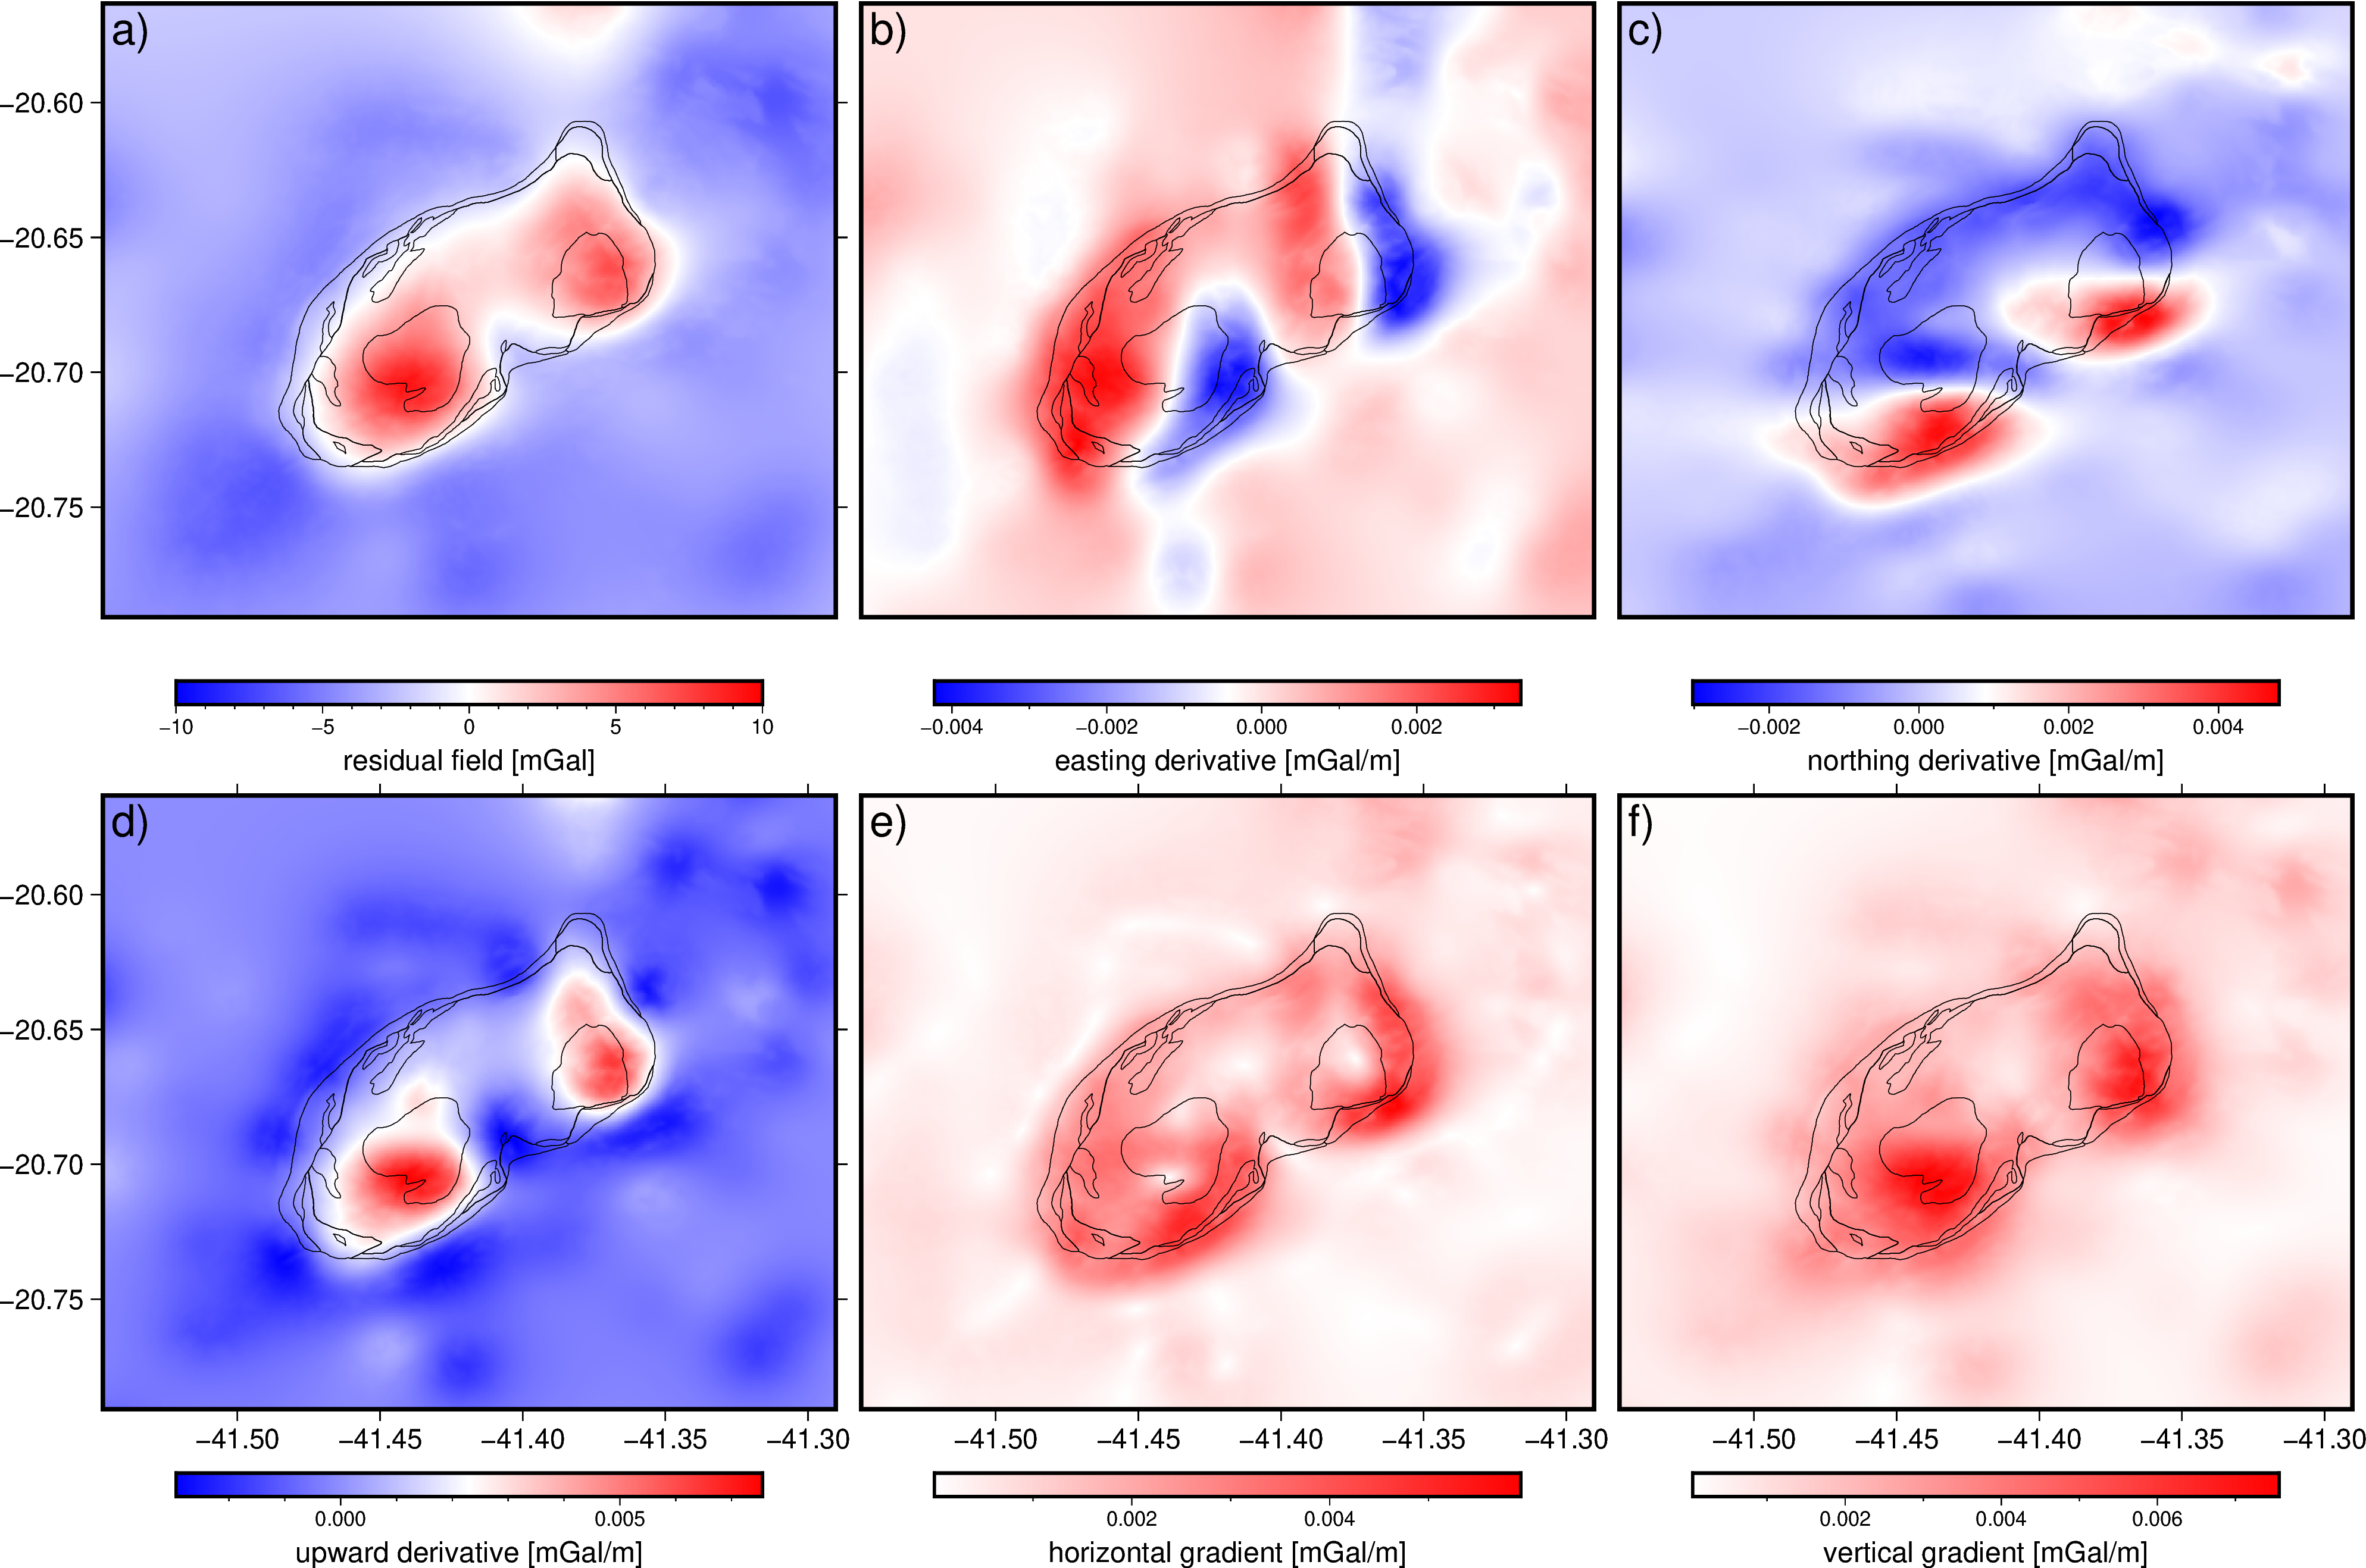
\includegraphics[width=1\linewidth]{figures/painel_final.png}
  \caption{
    Interpolated maps. a) Residual Bouguer disturbance. b) Horizontal gradient anomaly. c) Total gradient anomaly.
      }
  \label{final}
\end{figure}
